%************************************************
\chapter{Generative Adversarial Networks}
\label{chp:GANs}
%************************************************
Generative adversarial networks (GANs) (\cite{NIPS2014_5ca3e9b1}) have demonstrated great performance on producing realistic images, language, and even music. As deep \textit{generative} models, they were traditionally used in the context of unsupervised learning. However, this general technique has also been extended to other problems in semisupervised learning, such as image classification (\cite{denton2015deep, radford2015unsupervised}).\par
GANs learn the high-dimensional distribution of the unlabeled data through a pair of networks (the generator and the discriminator) that are competing against each other. An analogy is used in the original paper: the generator is a team of counterfeiters that produces fake currency, while the discriminator is the police trying to detect forgery. When both networks are optimal, the generator is able to produce counterfeit currency that is indistinguishable from the real ones.\par
In this section, we first provide an overview of GANs. Then, we will discuss their limitations, which leads to the section of \hyperref[chp:WGANs]{Wasserstein GANs}. Since the nature of this review is more mathematically motivated, for details on different GAN architecture and applications, see \cite{creswell2018generative}.
%% What is a GAN - how do they work
\section{Adversarial Nets}
    We define $p_z, p_g, p_r$ as the distributions of the latent variable $z$ (e.g. $z \sim \mathcal{N}(0,1)$), generator, and real samples respectively. The discriminator $D(x,\theta_d)$ outputs a scalar that represents the probability that $x$ came from $p_r$ rather than $p_g$. The generator $G(z, \theta_g)$ then learns a mapping from $z$ to the data space. In other words, it is learning $p_g$ over data $x$, where $x\sim p_r(x)$.\par
    \begin{figure}[htbp]
        \centering
        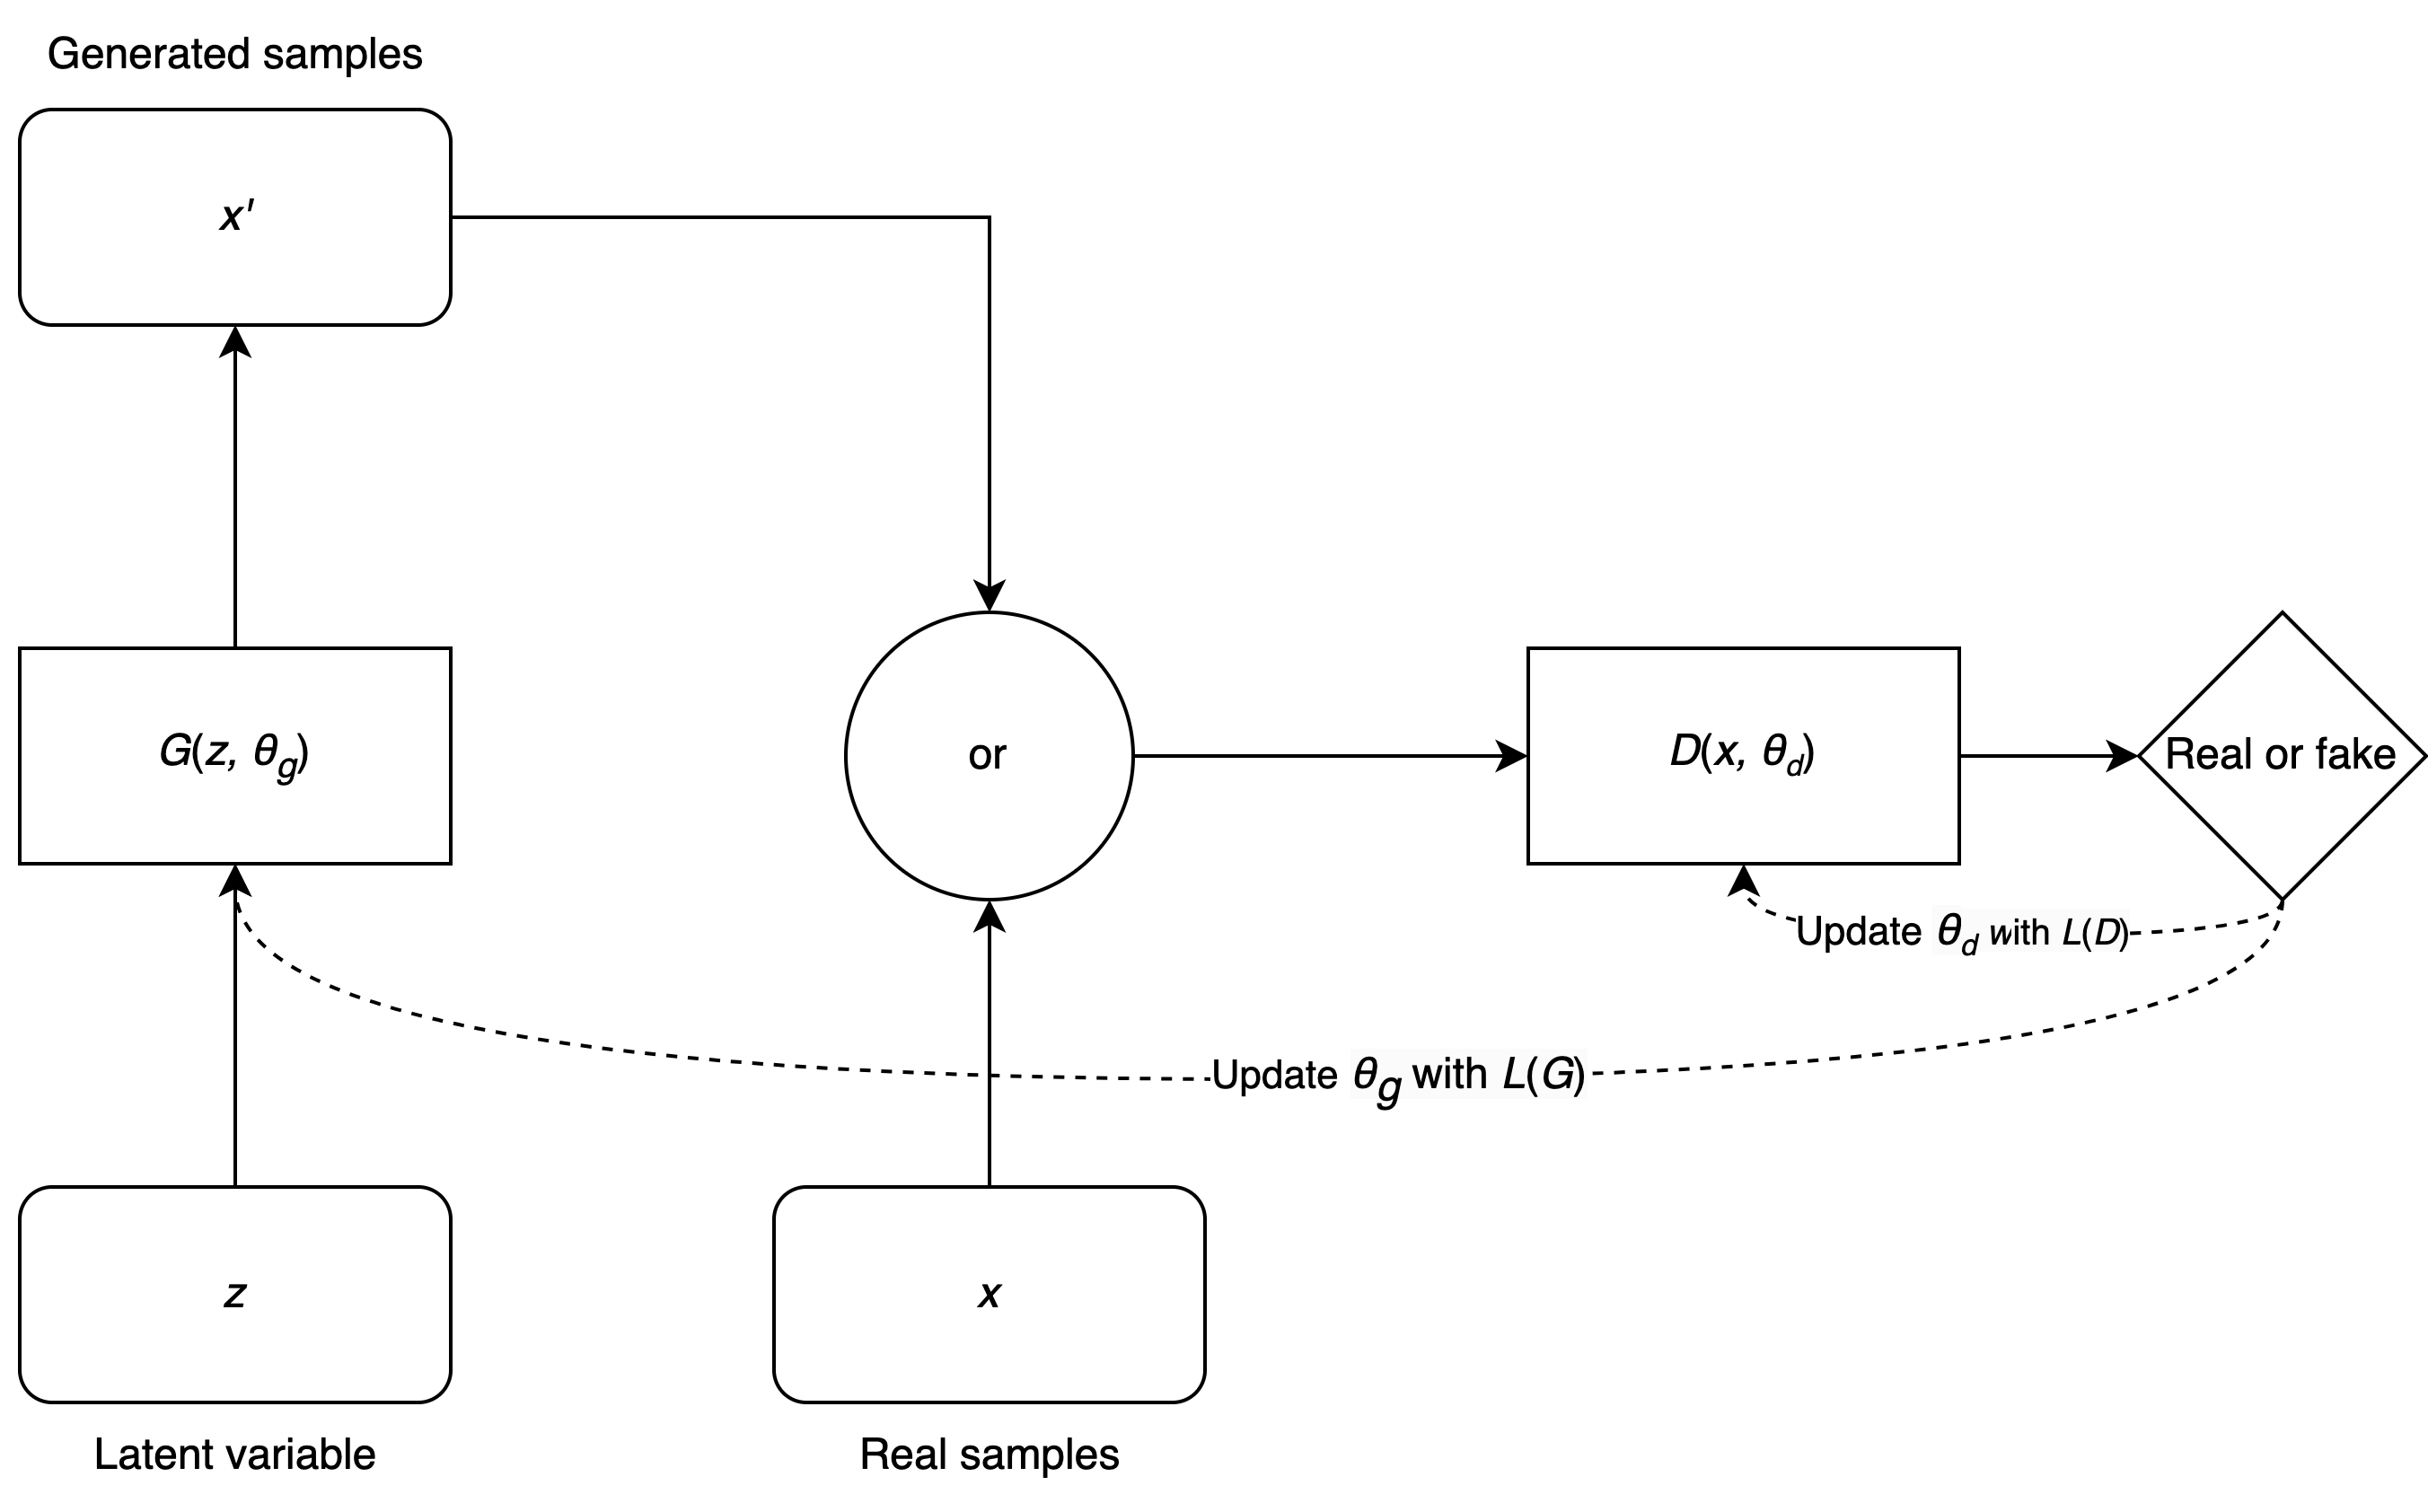
\includegraphics[width=0.6\linewidth]{Graphics/adver_net.png}
        \caption{A GAN consists of two models: a discriminator $D$ that outputs the probability that a given sample is real, and a generator $G$ that produces synthetic samples given a latent variable $z$ sampled from the base distribution. The discriminator parameters $\theta_d$ are updated to assigns high probability to real samples and low probability to synthetic samples. The generator parameters $\theta_g$ are updated to "fool" the discriminator into assigning high probabilities to the generated samples.}
        \label{fig:adv_net}
    \end{figure}
    $D$ is trained in a binary classification fashion; it maximizes the probability of assigning the correct label to both real samples $x$ and fake samples $x' = G(z)$. This is equivalent to maximizing $\mathbb{E}_{x\sim p_r(x)}\left[\log (D(x))\right] +\mathbb{E}_{z\sim p_z(z)}\left[\log(1- D(G(z)))\right]$. The generator then minimizes the probability of the discriminator assigning the correct label to the fake samples: $\mathbb{E}_{z\sim p_z(z)}\left[\log(1- D(G(z)))\right]$. In other words, they are playing a minimax game with the following loss function $L(G, D)$:
    \begin{equation}
        \min_{G}\max_{D} L(G, D) = \mathbb{E}_{x\sim p_r(x)}\left[\log (D(x))\right] +\mathbb{E}_{z\sim p_z(z)}\left[\log(1- D(G(z)))\right]
    \end{equation}
    \section{Training GANs}
    Since the discriminator and the generator are playing a two-player non-cooperative game, training them can be thought of as finding the Nash equilibrium, which can be difficult (\cite{salimans2016improved}). In practice, this is done by the following: in each training loop, fix the generator and update the discriminator for $k$ steps, then fix the discriminator and update the generator for 1 step. To update the discriminator, we use the following loss function\footnotemark{}\footnotetext{Equation \eqref{eq:dis_loss} is similar to the loss minimization function in \cite{prince2023understanding}. The original paper by \cite{NIPS2014_5ca3e9b1} uses minibatch stochastic gradient ascent for maximization.}:
    \begin{align}\label{eq:dis_loss}
        L(\theta_d) &= - \left(\mathbb{E}_{x\sim p_r(x)}\left[\log (D(x, \theta_d))\right] +\mathbb{E}_{z\sim p_z(z)}\left[\log(1- D(G^*(z), \theta_d))\right]\right)\notag\\
        &\approx -\frac{1}{m}\sum_{i=1}^m\left[\log (D(x_i, \theta_d))\right] - \frac{1}{n}\sum_{j=1}^n\left[\log(1-D(G^*(z_j), \theta_d))\right]
    \end{align}
    where $m$ represents the number of real examples, $n$ represents the number of fake examples, and $G^*(z)$ represents the fixed generator. To update the generator, we use the following loss function:
    \begin{align}\label{eq:gen_loss}
        L(\theta_g) &= \left(\mathbb{E}_{x\sim p_r(x)}\left[\log (D^*(x))\right] +\mathbb{E}_{z\sim p_z(z)}\left[\log(1- D^*(G(z, \theta_g)))\right]\right)\\
        &\approx \frac{1}{n}\sum_{j=1}^n\left[\log(1-D^*(G(z_j, \theta_g)))\right] \tag{first term is not related to $G(z, \theta_g)$}
    \end{align}
    where $D^*(x)$ represents the fixed generator. There are also interesting theoretical results related to the loss function of GANs, which have been used by others to analyze their limitations.
        \subsection{Optimal Value for Discriminator and Generator}
        Given a fixed generator $G^*(z, \theta_g)$, the goal is to maximize the loss function for the discriminator $D$:
        \begin{align}\label{eq:max_dis}
            L(G, D) &= \mathbb{E}_{x\sim p_r(x)}\left[\log (D(x))\right] +\mathbb{E}_{z\sim p_z(z)}\left[\log(1- D(G^*(z)))\right]\notag\\
            &= \mathbb{E}_{x\sim p_r(x)}\left[\log (D(x))\right] +\mathbb{E}_{x\sim p_g(x)}\left[\log(1- D(x)\right]\\
            &= \int_{x}p_r(x)\log(D(x))+ p_g(x)\log(1-D(x))dx\notag
        \end{align}
        The maximum value for this function is achieved when $D^*(x) = \frac{p_r(x)}{p_r(x)+p_g(x)}$, and when the \textit{generator} is trained to its optimal, $p_r = p_g$, so $D(x) = \frac{1}{2}$. This is equivalent to the optimal discriminator assigning random labels to any given sample. Although it is trained, it cannot distinguish between real and fake anymore.
        \subsection{Global Optimal and Relationship to JS Divergence}\label{sec:global_opt}
        Given $G^*(z, \theta_g)$ such that $p_r = p_g$, and $D^*(x, \theta_d)$ such that $D^*(x) = \frac{1}{2}$,
        \begin{align}\label{eq:global_optimal}
            L(G^*, D^*) &= \mathbb{E}_{x\sim p_r(x)}\left[-\log2\right] +\mathbb{E}_{x\sim p_g(x)}\left[-\log2)\right]\notag\\
            &= -2\log2
        \end{align}
        Thus, the best possible value of $L(G, D)$ is $-2\log2$.\par
        KL-divergence is defined as:
        \begin{equation}\label{eq:KL}
            KL(p\|q) = \int_{x}p(x)\log\frac{p(x)}{q(x)}dx
        \end{equation}
        and JS-divergence is defined as:
        $$
        JSD(p\|q) = \frac{1}{2}KL(p\|\frac{p+q}{2}) + \frac{1}{2}KL(q\|\frac{p+q}{2})
        $$
        Notice that when $D^*(x) = \frac{p_r(x)}{p_r(x)+p_g(x)}$ is used in equation \eqref{eq:max_dis}, it is equivalent to measuring the KL (Kullback-Leibler) divergence between $p_r, \frac{p_r+p_g}{2}$ and $p_g, \frac{p_r+p_g}{2}$, which can be further simplified into the JS (Jensen-Shannon) divergence between $p_r, p_g$:
        \begin{align*}
            L(G, D^*) &= \mathbb{E}_{x\sim p_r(x)}\left[\log (D^*(x))\right] +\mathbb{E}_{x\sim p_g(x)}\left[\log(1- D^*(x)\right]\\
            &= \int_{x}p_r(x)\log\left(\frac{2\cdot p_r(x)}{2\cdot(p_r(x)+p_g(x))}\right)dx+ \int_{x}p_g(x)\log\left(\frac{2\cdot p_g(x)}{2\cdot(p_r(x)+p_g(x))}\right)dx\\
            &= -2\log2 + \int_{x}p_r(x)\log\left(\frac{p_r(x)}{\frac{p_r(x)+p_g(x)}{2}}\right)dx+ \int_{x}p_g(x)\log\left(\frac{p_g(x)}{\frac{p_r(x)+p_g(x)}{2}}\right)dx\\
            &= -2\log2 + KL(p_r\|\frac{p_r+p_g}{2}) + KL(p_g\|\frac{p_r+p_g}{2})\\
            &= -2\log2 + 2JSD(p_r\|p_g)
        \end{align*}
        Thus, when the discriminator is optimal, the loss function is equivalent to measuring the difference between $p_g$ and $p_r$, which is how well the generator is performing. Also, when the generator is optimal, $p_r = p_g$, and $2JSD(p_r, p_g)=0$, so $L(G^*, D^*) = -2\log2$, which confirms equation \eqref{eq:global_optimal}.\par
        
        Some have suggested that the use of JS-divergence term in GAN's loss function is the reason behind its success. Since JS-divergence is symmetric, it would not penalize one distribution more than the other and cause "mode dropping". Specifically, consider the terms in equation \eqref{eq:KL} of $KL(p_r\|p_g)$: if $p_r(x)>p_g(x)$, then $x$ is more likely to come from the true data distribution. But when $p_r(x)>0, p_g(x)\to0$, KL-divergence becomes very large, so it over penalizes the generator for not covering parts of the true distribution. On the other hand, if $p_r(x)<p_g(x)$, and $p_r(x)\to0, p_g(x)>0$, then KL-divergence becomes very small, so it under penalizes the generator for generating fake looking samples.
%% Limitations of GANs (foreshadowing for WGANs)
\section{Limitations of GANs}
GANs were known to be difficult to train. Many approached this problem by relying on heuristics, and proposed techniques such as feature matching and minibatch discrimination (\cite{radford2015unsupervised, salimans2016improved}). While the techniques improved the stability of GANs in practice, these variants were very sensitive to modifications. \cite{arjovsky2017towards} provided a new perspective on GANs by introducing the theory behind their instability issues.

    \subsection{The Real Cost}
    Based on the analysis in \autoref{sec:global_opt}, the optimally trained discriminator should have maximum cost of $2\log2-2JSD(p_r\|p_g)$, and with the optimal generator, this cost goes to $2\log2$. However, in practice, this cost approaches $0$. This implies that $JSD(p_r\|p_g)=\log2$, and that the JS-divergence between the two distributions is maxed out. It is shown that this occurs because the supports for  $p_r$ and $p_g$ lie on low dimensional manifolds.\par
    To provide some intuition, consider the data space $\mathcal{X}$ which contains all the possible real-world images. Although the dimension of $\mathcal{X}$ appears to be artificially high, there are many pre-existing restrictions placed by nature. For instance, a mammal face usually contains eyes, ears, a nose, a mouth, and a jaw. Thus, the support of $p_r$ is concentrated on a low dimensional manifold. Similarly, the generator $G(z, \theta_g): \mathcal{Z} \to \mathcal{X}$ is defined by sampling from a prior distribution $p_z$, which has less dimension (such as 100) than $\mathcal{X}$.\par
    Recall that if $\mathcal{X}: \Omega\to\mathbb{R}^n$ is a random variable, then the support of $\mathcal{X}$ is defined as the set $R_x = \{x\in\mathbb{R}^n: p_r(x)>0\}$. For instance, the support of $p_g$ has to be contained in $G(z, \theta_g)$. Denote $\mathcal{M}$ as the manifold where the support of $p_r$ lies in, and $\mathcal{P}$ the manifold where the support of $p_g$ lies in. It can be shown that
    \begin{enumerate}
        \item \label{item:perfect_dis} If $\mathcal{M}$ and $\mathcal{P}$ don't perfectly align and don't have full dimensions, then there exists a perfect discriminator $D^{**}: \mathcal{X}\to[0,1]$ such that it takes the value $1$ on a set that contains the support of $p_r$ and value $0$ on a set that contains the support of $p_g$. Also, $\nabla_xD^*(x)=0$
        \item \label{item:infy_KL} If $\mathcal{M}$ and $\mathcal{P}$ don't perfectly align and don't have full dimensions, then
            \begin{align*}
                JSD(p_r\|p_g) &= \log2\\
                KL(p_r\|p_g) &= +\infty\\
                KL(p_g\|p_r) &= +\infty
            \end{align*}
        \item \label{item:grad_bound} Let $J_{\theta_g} G(z,\theta_g)$ denote the Jacobian of $G$ with respect to $\theta_g$. If \ref{item:perfect_dis} is satisfied, and $\|D-D^{**}\|<\epsilon$, and $\mathbb{E}_{z\sim p(z)}\left[\|J_{\theta_g} G(z,\theta_g)\|^2_2\right]\leq C^2$, then
        \begin{equation}
            \|\nabla_{\theta_g}\mathbb{E}_{z\sim p(z)}\left[\log(1-D(G(z,\theta_g)))\right]\|_2 < C\frac{\epsilon}{1-\epsilon}
        \end{equation}
    \end{enumerate}
    Note that the perfect discriminator $D^{**}$ in \ref{item:perfect_dis} is different from the optimal discriminator in \autoref{sec:global_opt}, which assigns equal probabilities to fake and real samples. In fact, this difference is precisely the reason why in practice, the cost of the discriminator approaches 0. In conjunction with the result in \ref{item:infy_KL}, we understand that although the generator is producing realistic looking results, the two underlying distributions $p_r, p_g$ are actually very different and easy for the discriminator to distinguish.\par
    \begin{figure}[htbp]
        \caption{Low dimensional manifolds in high dimension space can hardly have overlaps.}
        \centering
        \begin{tikzpicture}[scale=0.6]
            % axis
            \draw[ultra thick,->] (0.3,-3.5) -- +(0,7) node[yshift=5pt] {$y$};
            \draw[ultra thick,->] (0.3,-3.5) -- +(220:4) node[yshift=-5pt,xshift=-5pt] {$z$};
            \draw[ultra thick,->] (0.3,-3.5) -- +(12,0) node[xshift=6pt] {$x$};
            
            % border of the surface1
            \path[draw,name path=border1] (0,0) to[out=-10,in=150] (6,-2);
            % border of the surface1
            \path[draw,name path=border2] (12,1) to[out=150,in=-10] (5.5,3.2);
            % border of the surface1
            \draw[draw,thick,name path=line1] (6,-2) -- (12,1);
            % border of the surface1
            \path[draw,name path=line2] (5.5,3.7) -- (0,0);
            % draw the surface1
            \shade[left color=gray!10,right color=gray!70] 
              (0,0) to[out=-10,in=150] (6,-2) -- 
              (12,1) to[out=150,in=-10] (5.5,3.7) -- cycle;
            
            % border of the surface2
            \path[draw,name path=border3] (-1,-4) to[out=20,in=220] (3,3);
            % border of the surface2
            \path[draw,name path=border4] (6,-7) to[out=40,in=210] (9,1);
            % border of the surface2
            \path[draw,name path=border5] (-1,-4) to[out=0,in=80] (6,-7);
            % border of the surface2
            \path[draw,name path=border6] (3,3) to[out=10,in=140] (9,1);
            
            % labels
            \node at (0.5,-3.8) {$p_r$};
            \node at (10,1) {$p_g$};
            
            % draw the surface2
            \shade[top color=gray!10,bottom color=gray!90,opacity=.30] 
              (-1,-4) to[out=20,in=220] (3,3)  to[out=10,in=140] (9,1)
             to[out=210,in=40] (6,-7) to[out=80,in=0] (-1,-4);
            
            % intersection points
            \path[name intersections={of=border3 and line2,by={a}}];
            \path[name intersections={of=border4 and line1,by={b}}];
            
            % intersection of the surfaces
            \draw[thick,dashed] (a) to[out=-10,in=130] (b);
        \end{tikzpicture}
        \label{fig:manifold}
    \end{figure}
    To explain the idea in \ref{item:infy_KL} in simpler terms, imagine the following four cases between $p_r$ and $p_g$ when calculating $JSD$: 
    \begin{align*}
        p_r(x) &= 0, p_g(x) = 0\\
        p_r(x) &\neq 0, p_g(x) \neq 0\\
        p_r(x) &= 0, p_g(x) \neq 0\\
        p_r(x) &\neq 0, p_g(x) = 0
    \end{align*}
    The first case does not contribute to $JSD$. The third case is $\frac{1}{2}\log\left(\frac{p_r}{\frac{p_r+0}{2}}\right)=\frac{1}{2}\log2$ in $JSD$ calculation. Similarly, the fourth case contributes $\frac{1}{2}\log2$. For the second case, since $\mathcal{M}$ and $\mathcal{P}$ don't perfectly align and don't have full dimensions, for any parts where $p_r(x)$ and $p_g(x)$ overlap, the resulting integral is negligible, so it also does not contribute to $JSD$. To provide further intuition, if the data space is $\mathbb{R}^3$, and the supports are planes, then it is very unlikely for them to be perfectly aligned; their intersection is most likely a line which does not contribute to the measure (see \autoref{fig:manifold}).\par 
    Finally, the result in \ref{item:grad_bound} provides a bound on the generator's loss when the difference between the discriminator and the perfect discriminator is small. In fact, when the discriminator is perfect, the gradient provided to the generator approaches $0$. This is intuitive as the generator loss function (\autoref{eq:gen_loss}) depends on the discriminator.
    $$\lim_{\|D-D^{**}\|\to0}\nabla_{\theta_g}\mathbb{E}_{z\sim p(z)}\left[\log(1-D(G(z,\theta_g)))\right] = 0$$
    This is also known as the vanishing gradient problem, and explains the instability behaviour in GAN training.  Overall, this subsection shows that under the original loss function, there exists a perfect discriminator, which easily distinguishes $p_g,p_r$, and provides little signal for the generator to learn.
    \subsection{Ways to Address the Instability}
    In the original paper (\cite{arjovsky2017towards}), the authors first proposed to add noise to $p_r$ and $p_g$ such that their manifolds are able to "spread" to the higher dimensions such that the measure of their overlaps is more significant in higher dimensions. During training, this added noise can be gradually removed, until eventually, the two manifolds are perfectly aligned.\par 
    However, they also proposed to use another metric that directly measures the distance between points in the manifolds. This is known as the Wasserstein distance.
    